\section{Large Scale Structure \Contact{Tony}}
\Contributors{Tony, Rogerio,...}
\label{sec:lss}

\begin{figure}[t]
\centering
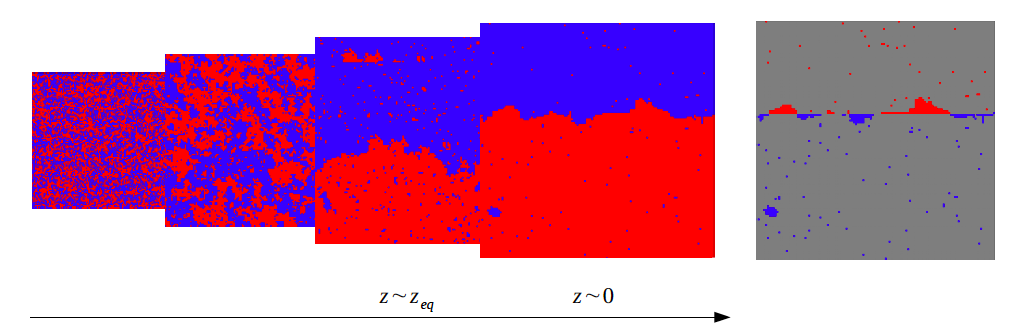
\includegraphics[width=0.9\columnwidth]{DMDE-anisotropy.png}
\caption{A schematic diagram of the emergence of dark energy anisotropy from an Ising model phase transition and a coupling with the anisotropic distribution of dark matter. Figure taken from \citet{1810.11007}.}
\label{fig:DMDEmap}
\end{figure}

The physics of dark matter could be probed via LSST if dark energy were an aspect of dark matter at late times. 
The natural inhomogeneities in dark matter on large scales would then be reflected as spatial inhomogeneities in the developing late-time acceleration. 
This could be observed as spatial variations in cosmic acceleration by LSST correlated with the large scale dark matter weak lensing maps. 
Such a spatial correlation is a generic prediction if dark matter and dark energy are causally related or if dark energy is emergent \citep{1801.09658}. 
A spatially complicated potential leads to a small cosmological constant from an energy difference between its global and local minima, and dark energy and dark matter are thereby intertwined. 
If so, and if the universe on sub-horizon scales is not homogeneous, then spatial fluctuations in one component should be correlated with spatial fluctuations in the other, particularly near the epoch of emergence.

There are other models where dark matter and dark energy are intertwined, such as models where they interact 
\citep{Amendola:1999er,Holden:1999hm}.
Interacting models can be described phenomenologically via two fluids that can exchange energy and momentum, 
described by energy-momentum tensors that are not individually conserved. One can parameterize the coupling of
dark matter and dark energy by writing the divergence of the individual energy-momentum tensors as 
\begin{eqnarray}
\nabla_{\mu} T^{(DE)}\,^{\mu}_{\nu} &=& C^{(DE)}_{\nu}, \label{cons_phi} \\
\nabla_{\mu} T^{(DM)}\,^{\mu}_{\nu} &=& C^{(DM)}_{\nu}, \label{cons_dm}
\end{eqnarray}
where the superscript $(DM)$ stands for the dark matter fluid and $(DE)$ for the dark energy.
The conservation of the total dark component energy-momentum tensor 
(we assume the separate conservation of the energy momentum of radiation and baryons),
\begin{equation}
\label{energyconservation}
\nabla_{\mu} \left[ T^{(DM)} \,^{\mu}_{\nu} + T^{(DE)} \,^{\mu}_{\nu} \right]= 0,
\end{equation}
implies that
\begin{equation}
C^{(DM)}_{\nu}=-C^{(DE)}_{\nu}.
\end{equation}

The coupling between dark matter and dark energy is determined by the function $C^{(DM)}_{\nu}$ which is usually
written as
\begin{equation}
C^{(DM)}_{\nu} = (8\pi G)^{1/2} \,\beta\rho_{DM}\nabla_{\nu} \phi,
\end{equation}
where $\beta$ is a constant that expresses the coupling strength. In this model, dark energy must be dynamical and here it is modeled by a scalar field  $\phi$, such as a quintessence field.
In this model, $\beta$ is the only new parameter in addition to the usual description of the dark energy sector.
The standard uncoupled case is recovered for $\beta=0$.

There is a vast literature studying this class of models that can modify both the evolution of the 
background cosmology as well as the evolution of perturbations. For instance, it has been recently claimed
that such a model can ease the tension in the measurements of $\sigma_8$ from CMB and galaxy surveys 
\citep{Barros:2018efl}.

LSST can separately map dark matter and dark energy at a redshift where they have roughly comparable influences on the expansion rate of the universe. 
There are two complementary methods of reconstructing dark energy on the sky: SNe and 3$\times$2pt in 20 degree patches \citep[Figure 15.9 in ][]{0912.0201}.
The transition between a dark matter-dominated universe to one with late-time acceleration (dark energy) may hint at some connection between these two components. 
An angular cross correlation between maps of dark energy and tomographic weak lens maps of dark matter could yield a non-zero signal.  
If so, the ratio of the cross correlation to the auto-correlations would be a diagnostic of the underlying physics. 
In this scenario, measurements of dark energy anisotropy become a probe of the nature of dark matter; \figref{DMDEmap}, reproduced from \cite{1810.11007}, illustrates a Ginzburg-Landau phase transition model that results in correlated dark matter-dark energy anisotropy. 
Quadrupole and higher-order correlated anisotropies are generated around redshift $z=0.7$.  
This is accessible in LSST maps of dark energy and dark matter in a broad redshift shell.

\paragraph{Systematics and synergies:}
Systematics in the dark energy and dark matter maps on large angular scales must be reduced below the level of any dark matter-dark energy correlation signal.  
For example, systematics in apparent magnitude and \photoz due to uncorrected extinction from Galactic dust would be one focus. 
Encouragingly, the two measures of dark energy anisotropy depend differently on wavelength-dependent extinction. 
A useful null test will be the cross correlation between dark energy and dark matter maps with dust maps.  
This would set the floor for residual extinction systematics, forming the basis for a forward simulation of the resulting dark energy-dark matter false correlation. 
As in analysis of CMB data, cuts on Galactic latitude can reveal the level of residual systematics. 
Finally, any dependence of the cross-correlations on redshift could discriminate between models as well as detect redshift-dependent systematics.

For detection of low multipole sky correlations, observations in the north as well as the south will be useful.
There is important synergy with WFIRST and EUCLID observations in the north.  
These complementary data could be calibrated and tested by joint null tests in overlap areas with the LSST survey.